%%==================================================
%% chapter03.tex for TJU Master Thesis
%% Encoding: UTF-8
%%==================================================

\chapter{软管组件拉伸实验}
\section{引~言}
对软管组件进行拉伸实验,而不是进行内压实验,这是一个综合考虑各方面因素的结果。
首先,进行实验的目的是为了得到准确可靠的数据,以支撑理论模型,这就要求实验环境安全、可控,干扰的变量较少,所需数据如编织角、伸长量可以直接测量。
进行拉伸实验所需要的设备仅为力学万能试验机,安全可控,容易操作。
如果进行内压实验,实验的操作就必须在液压实验台上进行。根据试件的性能,内压荷载需要达到几十兆帕才能发生明显可测的变形。
%学者实验 研究
整个过程风险较大,液压试验台必须加盖隔离保护操作人员,因而液压实验中不能直接接触试件,需要通过额外的设备进行观测。

本文进行了三次拉伸实验,一方面是为了消除实验的系统误差,提高数据的可信度;另一方面,也是由于在理论研究过程中,发现了额外需要关注的部分、对象,也是一个循序渐进的探索过程。本章将着重介绍实验的结果以及对其结果的分析。
\section{观测数据及方法}


\subsection{编织角}
在实验过程中记录编织角并不简单,例如 ,本研究原计划采用摄像法记录软管组件编织角的变化,但由于软管编织层为为曲面,用平面的照片来进行编织角的采样,效果并不理想。测量的结果误差一般在$ \pm $2\textdegree 左右;整个拉伸实验过程中编织角的变化约为20\textdegree 。因此简单的摄像测量法相对误差保守估计在10\%左右。而且,产生误差的因素也很多,包括摄像设备与试件的相对位置,照片成像的质量,测量采样的位置等。因此国外有研究专门开发了记录编织角变化的试验台设备, \citeauthor{Leung2013}\cite{Leung2013}开发了双显微镜头的光学记录设备,
如\ref{fig:dic}图所示,配有伺服驱动装置,可以随着拉伸的过程同步移动,观测某一定点的编织角变化;并采用了数字图像处理技术(digital image corelation, DIC)对观测的结果进行处理,消除了曲面以及摄像角度的影响。

\begin{figure}[!htb]
	\centering
	\subfigure[]{
		\includegraphics[width=0.5\linewidth]{figure/experiment/dic-1}}		
	\hspace{1cm}
	\subfigure[]{
		\includegraphics[width=0.4\linewidth]{figure/experiment/dic-2}}
	\fcaption{数字化编织角观测设备}{DIC system of braid angle}
	\label{fig:dic}
\end{figure}

本研究由于设备有限,因而采用了另外一种处理方案来解决以上的问题。通过对目标区域进行染色处理,如图 所示,利用编织层表面凹凸不平的特性,趁染色涂料未干之际将编织角拓印在纸张上。

文献未见有类似的方法。从结果上来看,拓印法取得的编织角效果令人满意。拓印的编织纹路如图 所示,可以手工处理,也可通过电脑扫描后利用DIC软件处理,相比复杂的三位结构和空间几何透视关系,这种平面的纹路显然要更加容易处理。













\begin{figure}[!htb]
	\centering
	\subfigure[]{
		\includegraphics[height=0.2\textheight]{"figure/experiment/hose-angle-testing"}}		
	\hspace{1cm}
	\subfigure[]{
		\includegraphics[height=0.2\textheight]{"figure/experiment/hose-angle-testing-2"}}
	\fcaption{占位图}{place holder}
%	\label{fig:placeholder}
\end{figure}

%\subsubsection{拓印法步骤}

根据实验的经验,拓印记录编织角的纹路后,手工处理数据需要以下几步操作:
\begin{compactenum}
\item 观察两组不同方向的纹路,绘制两条参考线,保证分别与两个方向的纹路保持平行;
\item 测量不同数据点同荷载状态下,拓印纹路的参考线的夹角,计算平均值;
\item 若某组参考线的夹角明显不同于其余数据点,观察参考线绘制是否有误。
\end{compactenum}





\subsection{管径}
拉伸试验中,软管组件的管径会变小,是一个变化较明显的参数。管径测量较为简便,实验中采用游标卡尺即可测量。同样需要在测量编织角的数据点多次测量,过程中也要进行测量。
管径的作用主要是用以衡量标定有限元模型。
\subsection{支座反力与伸长量}
支座反力由试验机测得,一般不需要人为干预,软硬件都相对成熟。需要注意的时一般万能试验机可以记录的数据种类非常丰富,本实验中仅需记录支座反力与支座位移的关系曲线。
一般最大荷载较小的万能试验机测量精度较高,合理地选择试验机,将能得到更为准确的数据。







\section{实验设备}

力学万能试验机


\begin{figure}[!htb]
	\centering
	\subfigure[]{
		\includegraphics[height=0.22\textheight]{figure/experiment/tensile-machine}}		
	\hspace{1cm}
	\subfigure[]{
		\includegraphics[height=0.22\textheight]{figure/experiment/tensile-machine-2}}
	\fcaption{占位图}{place holder}
%	\label{fig:placeholder}
\end{figure}



\begin{figure}[!htb]
	\centering
	\subfigure{
		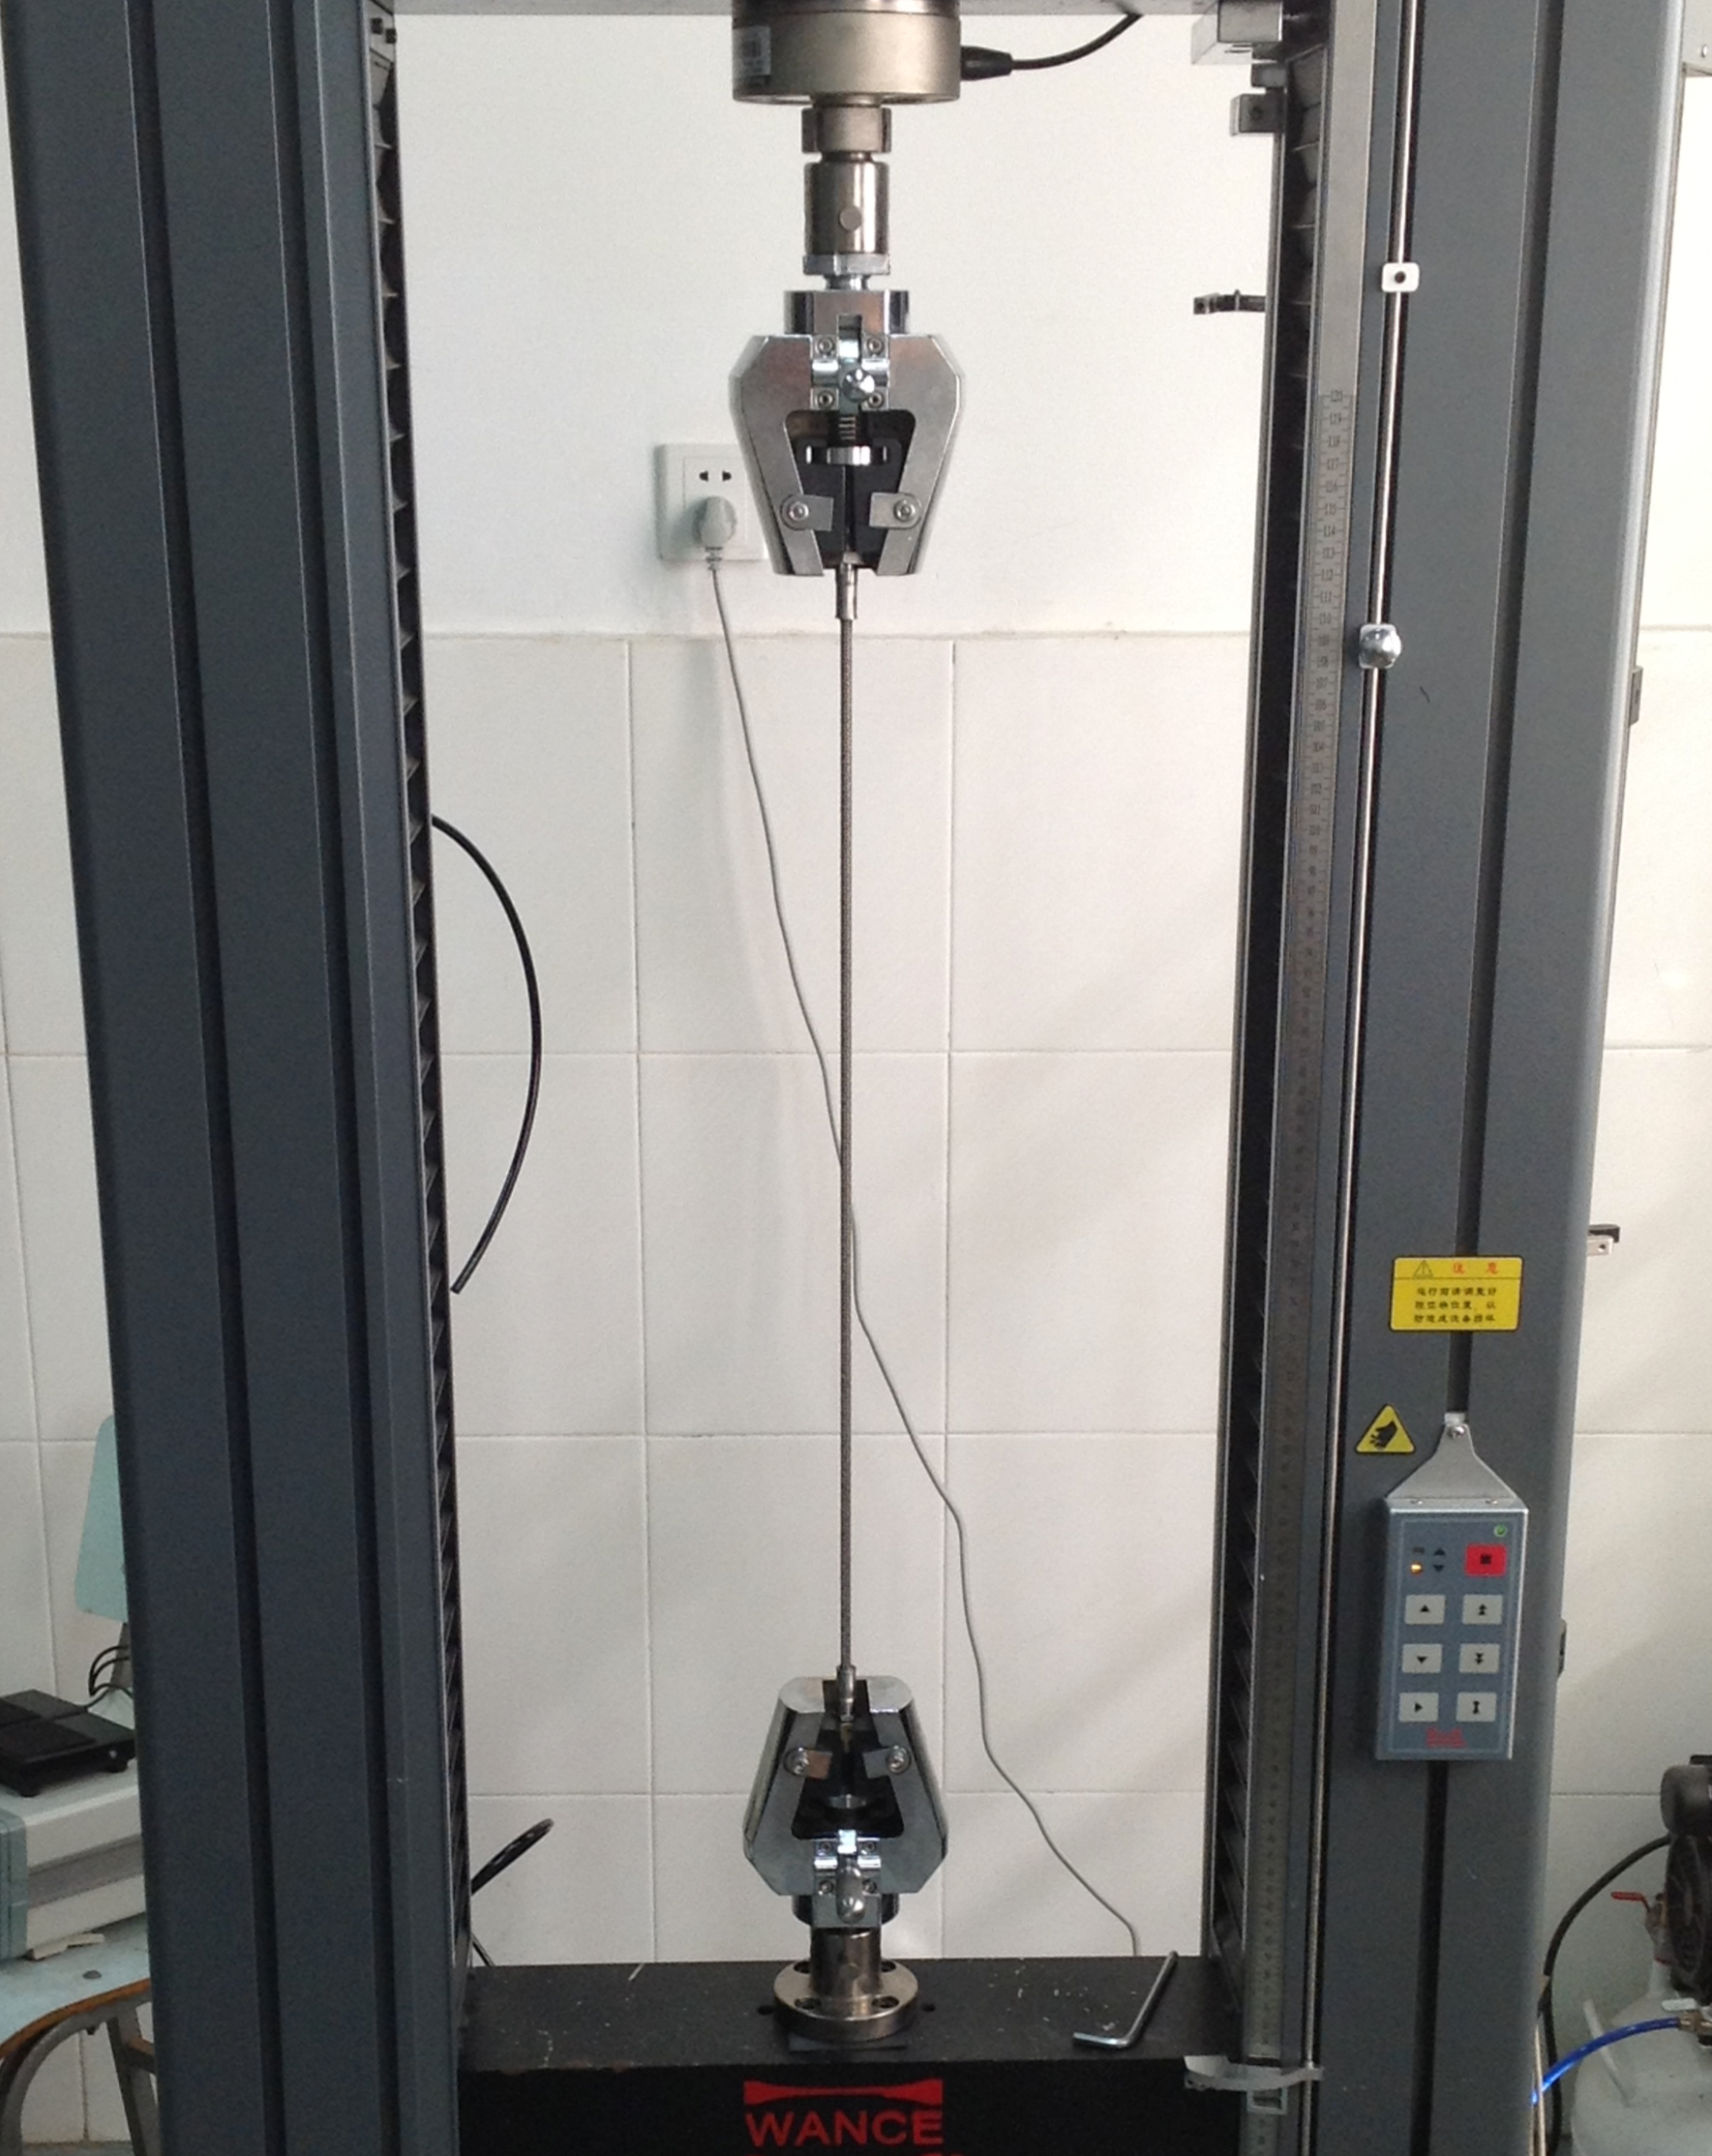
\includegraphics[height=0.3\textheight]{figure/experiment/tensile}
		\label{experiment-1}
	}
	\hspace{1cm}
	\subfigure{
		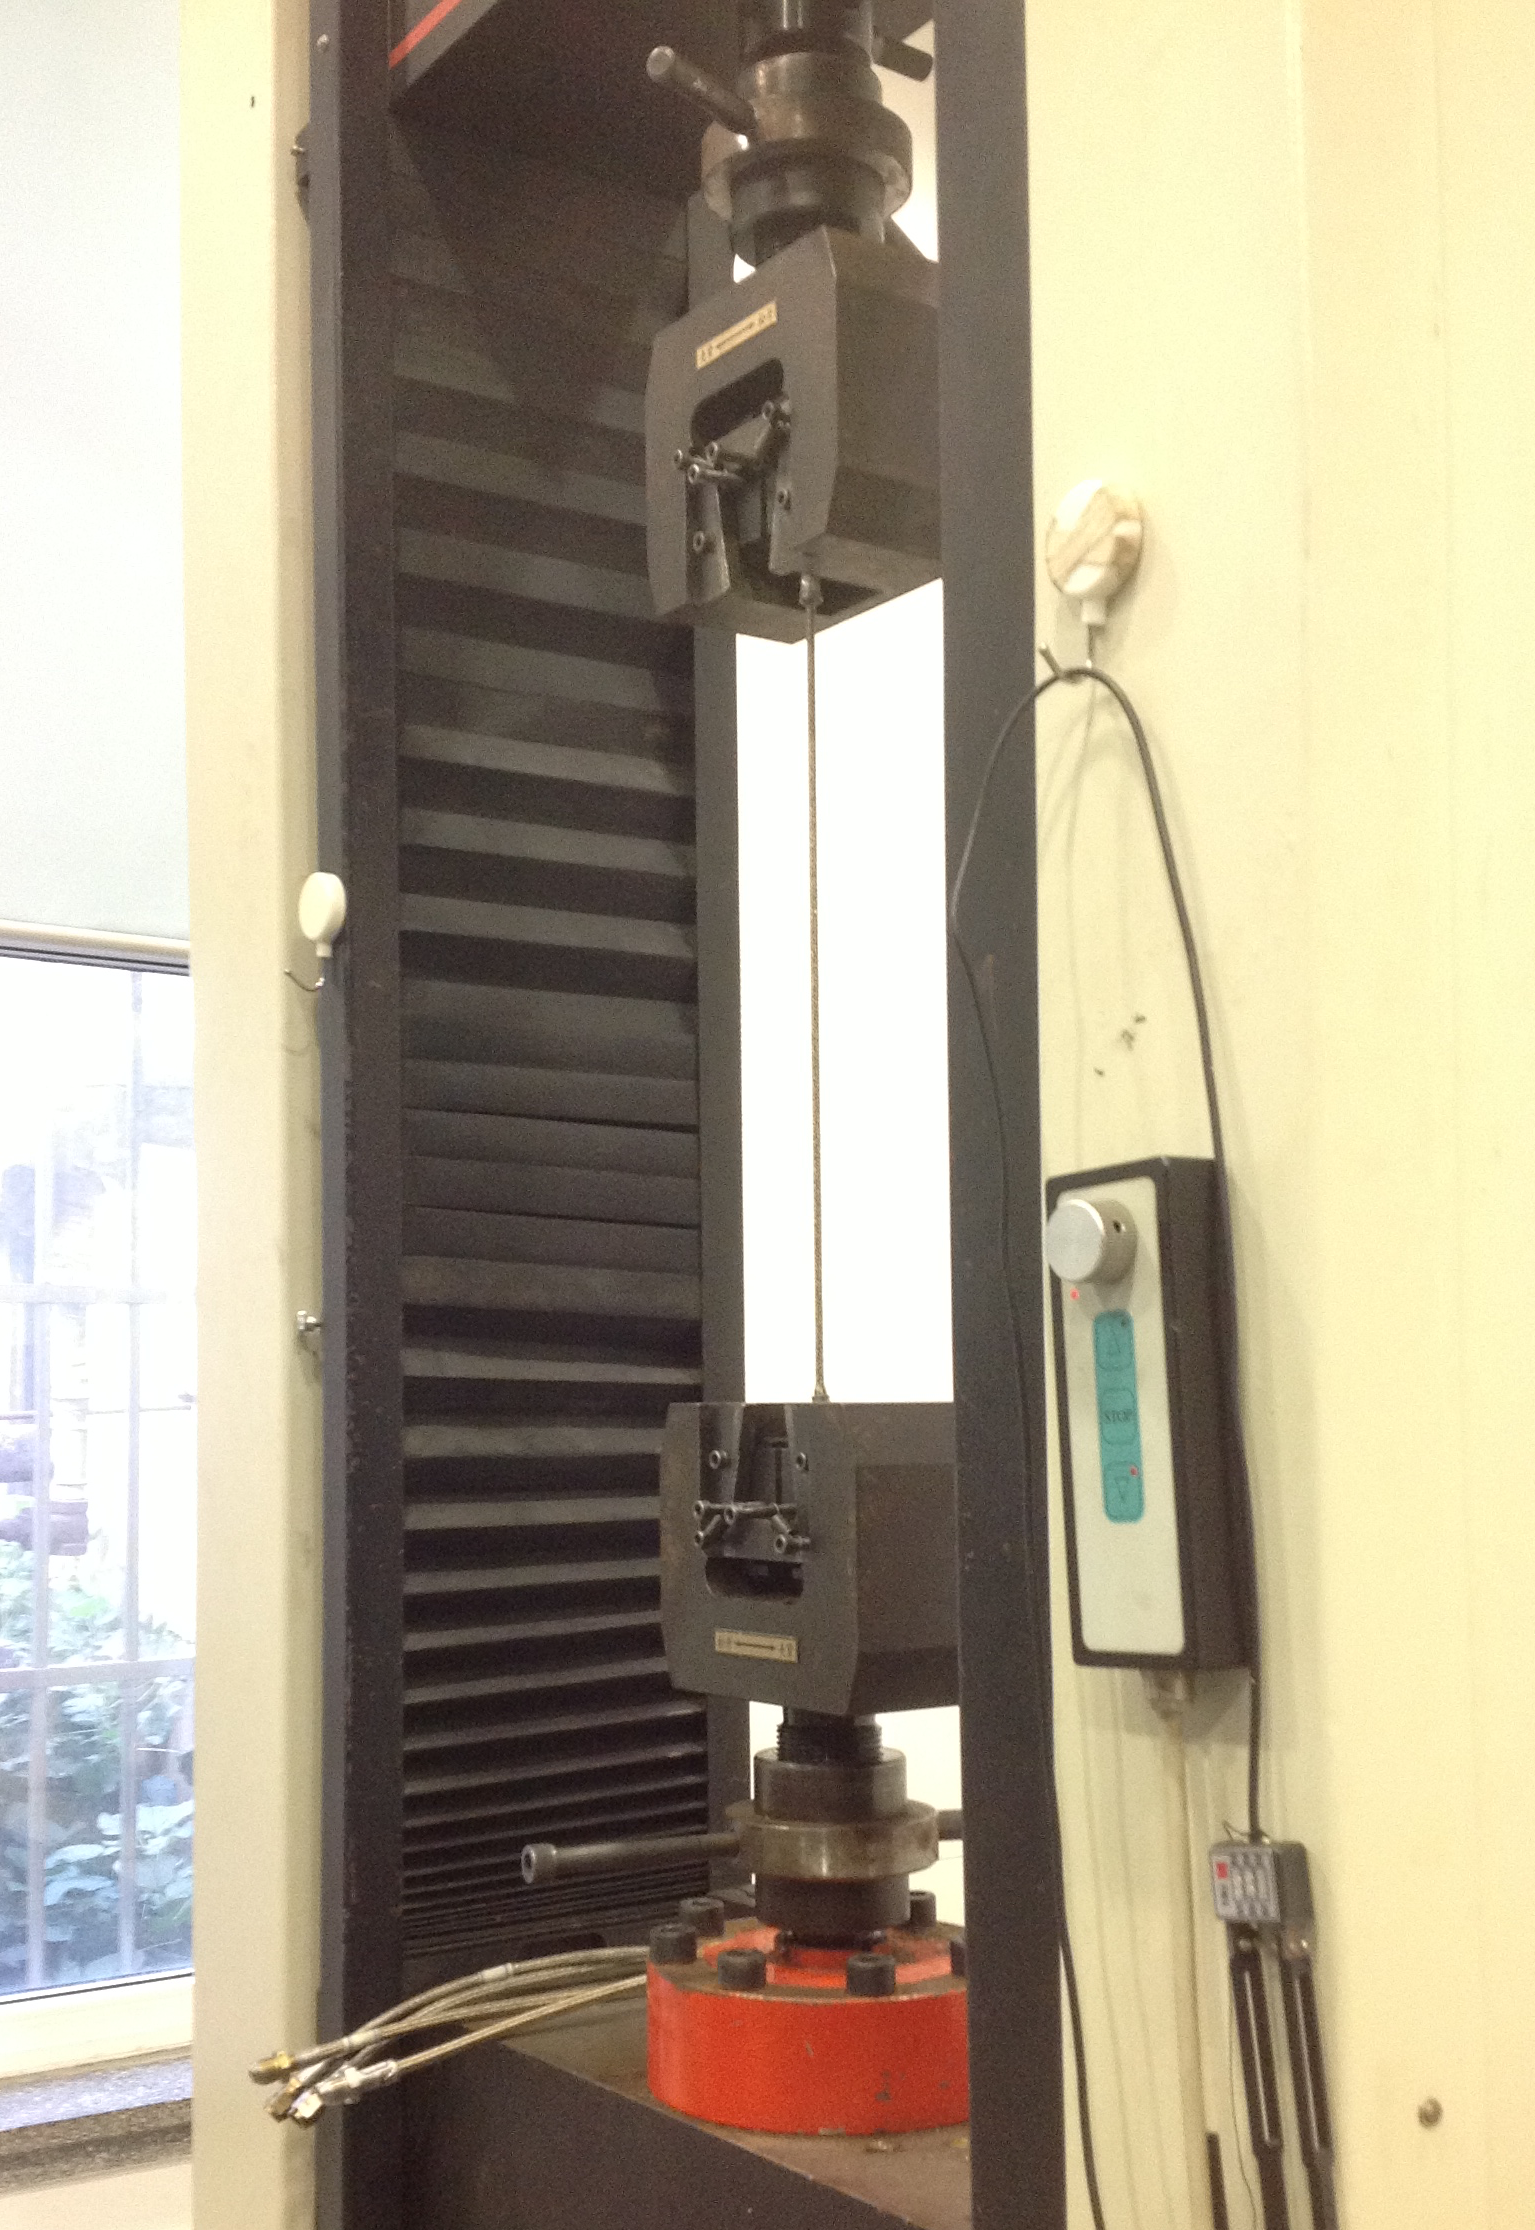
\includegraphics[height=0.3\textheight]{figure/experiment/experiment-1}
		\label{experiment-2}
	}

	\fcaption{拉伸实验}{experiments}  
	\label{fig:experiment}
\end{figure}



\section{实验步骤}

\begin{compactenum}
	\item 将软管安装至万能试验机,一般软管组件的的接头较为粗大,需要通过公装连接试验机夹具;
	\item 开始拉伸实验,加载速度不能超过10mm/min;
	\item 工程应变每增加0.05,至少记录一组数据,
	\begin{compactitem}
		\item 支座反力和软骨啊伸长量有试验机系统记录;
		\item 用拓印法记录编织角,至少3个染色区域,分别拓印记录;
		\item 记录染色区域的管径变化;
		\item 记录数据时拉伸的过程不会停止,必须短时间内测量记录各组数据,保证数据具有可比性。
	\end{compactitem}
	\item 试件破坏,实验结束。
\end{compactenum}





\section{第一次拉伸实验}
\subsection{试件参数}
 实验试件如图\ref{fig:experiment-1-specimen}所示。试件分别编号为芯棒1、芯棒2、芯棒3,芯棒4,共4组。
 “芯棒”代表试件制备的方法:编织机直接在将钢丝编织在芯棒上,然后抽出芯棒,仅保留编织层连接接头工装。
由于抽拔芯棒的过程,各组试件的编织角大幅小于平衡角。



\begin{figure}[!htb]
	\centering
	\subfigure[]{
		\includegraphics[width=0.35\textwidth]{figure/experiment/E1/specimen/E1-1}}
	\hspace{1cm}
	\subfigure[]{
		\includegraphics[width=0.35\textwidth]{figure/experiment/E1/specimen/E1-2}}
	
	\subfigure[]{
		\includegraphics[width=0.35\textwidth]{figure/experiment/E1/specimen/E1-3}}
	\hspace{1cm}
	\subfigure[]{
		\includegraphics[width=0.35\textwidth]{figure/experiment/E1/specimen/E1-4}}
	\fcaption{第一次拉伸实验}{experiment-1}  
	\label{fig:experiment-1-specimen}
\end{figure}

\begin{table}[!htb]
	\centering
	\tcaption{实验试件}{Hose Specimen of the traction experiment}
	\label{tab:hose-specimen}
	\begin{tabular*}{0.8\textwidth}{@{\extracolsep{\fill}}>{\hspace{0.5cm}}cccc}
		\toprule
		                  &     编织层-1     &     编织层-2     &     编织层-3     \\ \midrule
		外径(mm)            &     7.60      &     7.59      &     7.60      \\
		内径 (mm)           &     6.80      &     6.77      &     6.81      \\
		长度 (mm)           &     320.0     &     321.0     &     320.5     \\
		编织角 (\textdegree) &     42.1      &     41.9      &      43       \\
		股数$ \times $根数    & 24$ \times $6 & 24$ \times $6 & 24$ \times $6 \\
		钢丝直径(mm)          &      0.2      &      0.2      &      0.2      \\ \bottomrule
	\end{tabular*} 
\end{table}













\subsection{力位移曲线}
实验结果如图\ref{fig:experiment-results-1}所示,图为拉伸支座反力和拉伸量之间的关系,下文统一称之为“力-位移曲线”。
第一次拉伸实验共准备四组试件,对其中3组进行了拉伸实验。试件Hose-1拉伸至接头钢丝断裂破坏,Hose-2、Hose-3并未拉伸至破坏。观察三组拉伸实验的力-位移曲线结果,Hose-2与Hose-1的前段几乎完全重合;三组试件的结果趋势,大小一致,可见试件的质量、力学性质稳定,实验结果可信;实验结果中体现的编织层在应变较大时变现出来的高度的非线性,与\citeauthor{Hachemi2011}文献中的结果比较类似。

\begin{figure}[!htb]
	\centering
	\includegraphics[width=0.6\textwidth]{figure/experiment/E1/Graph01}
	
	\subfigure[]{
		\includegraphics[width=0.3\linewidth]{figure/experiment/E1/Graph03}}
	\subfigure[]{
		\includegraphics[width=0.3\linewidth]{figure/experiment/E1/Graph04}}
	\subfigure[]{
		\includegraphics[width=0.3\linewidth]{figure/experiment/E1/Graph05}}
	
	\fcaption{第一次拉伸实验}{experiment-1}  
	\label{fig:experiment-results-1}
\end{figure}



\subsection{破坏形式}

编织层试件拉伸过程中,接头处会发生颈缩的现象,最终也在接头处发生断裂破坏,如\ref{fig:experiment-1-fail}所示。



\begin{figure}[!htb]
	\centering
	\subfigure{
		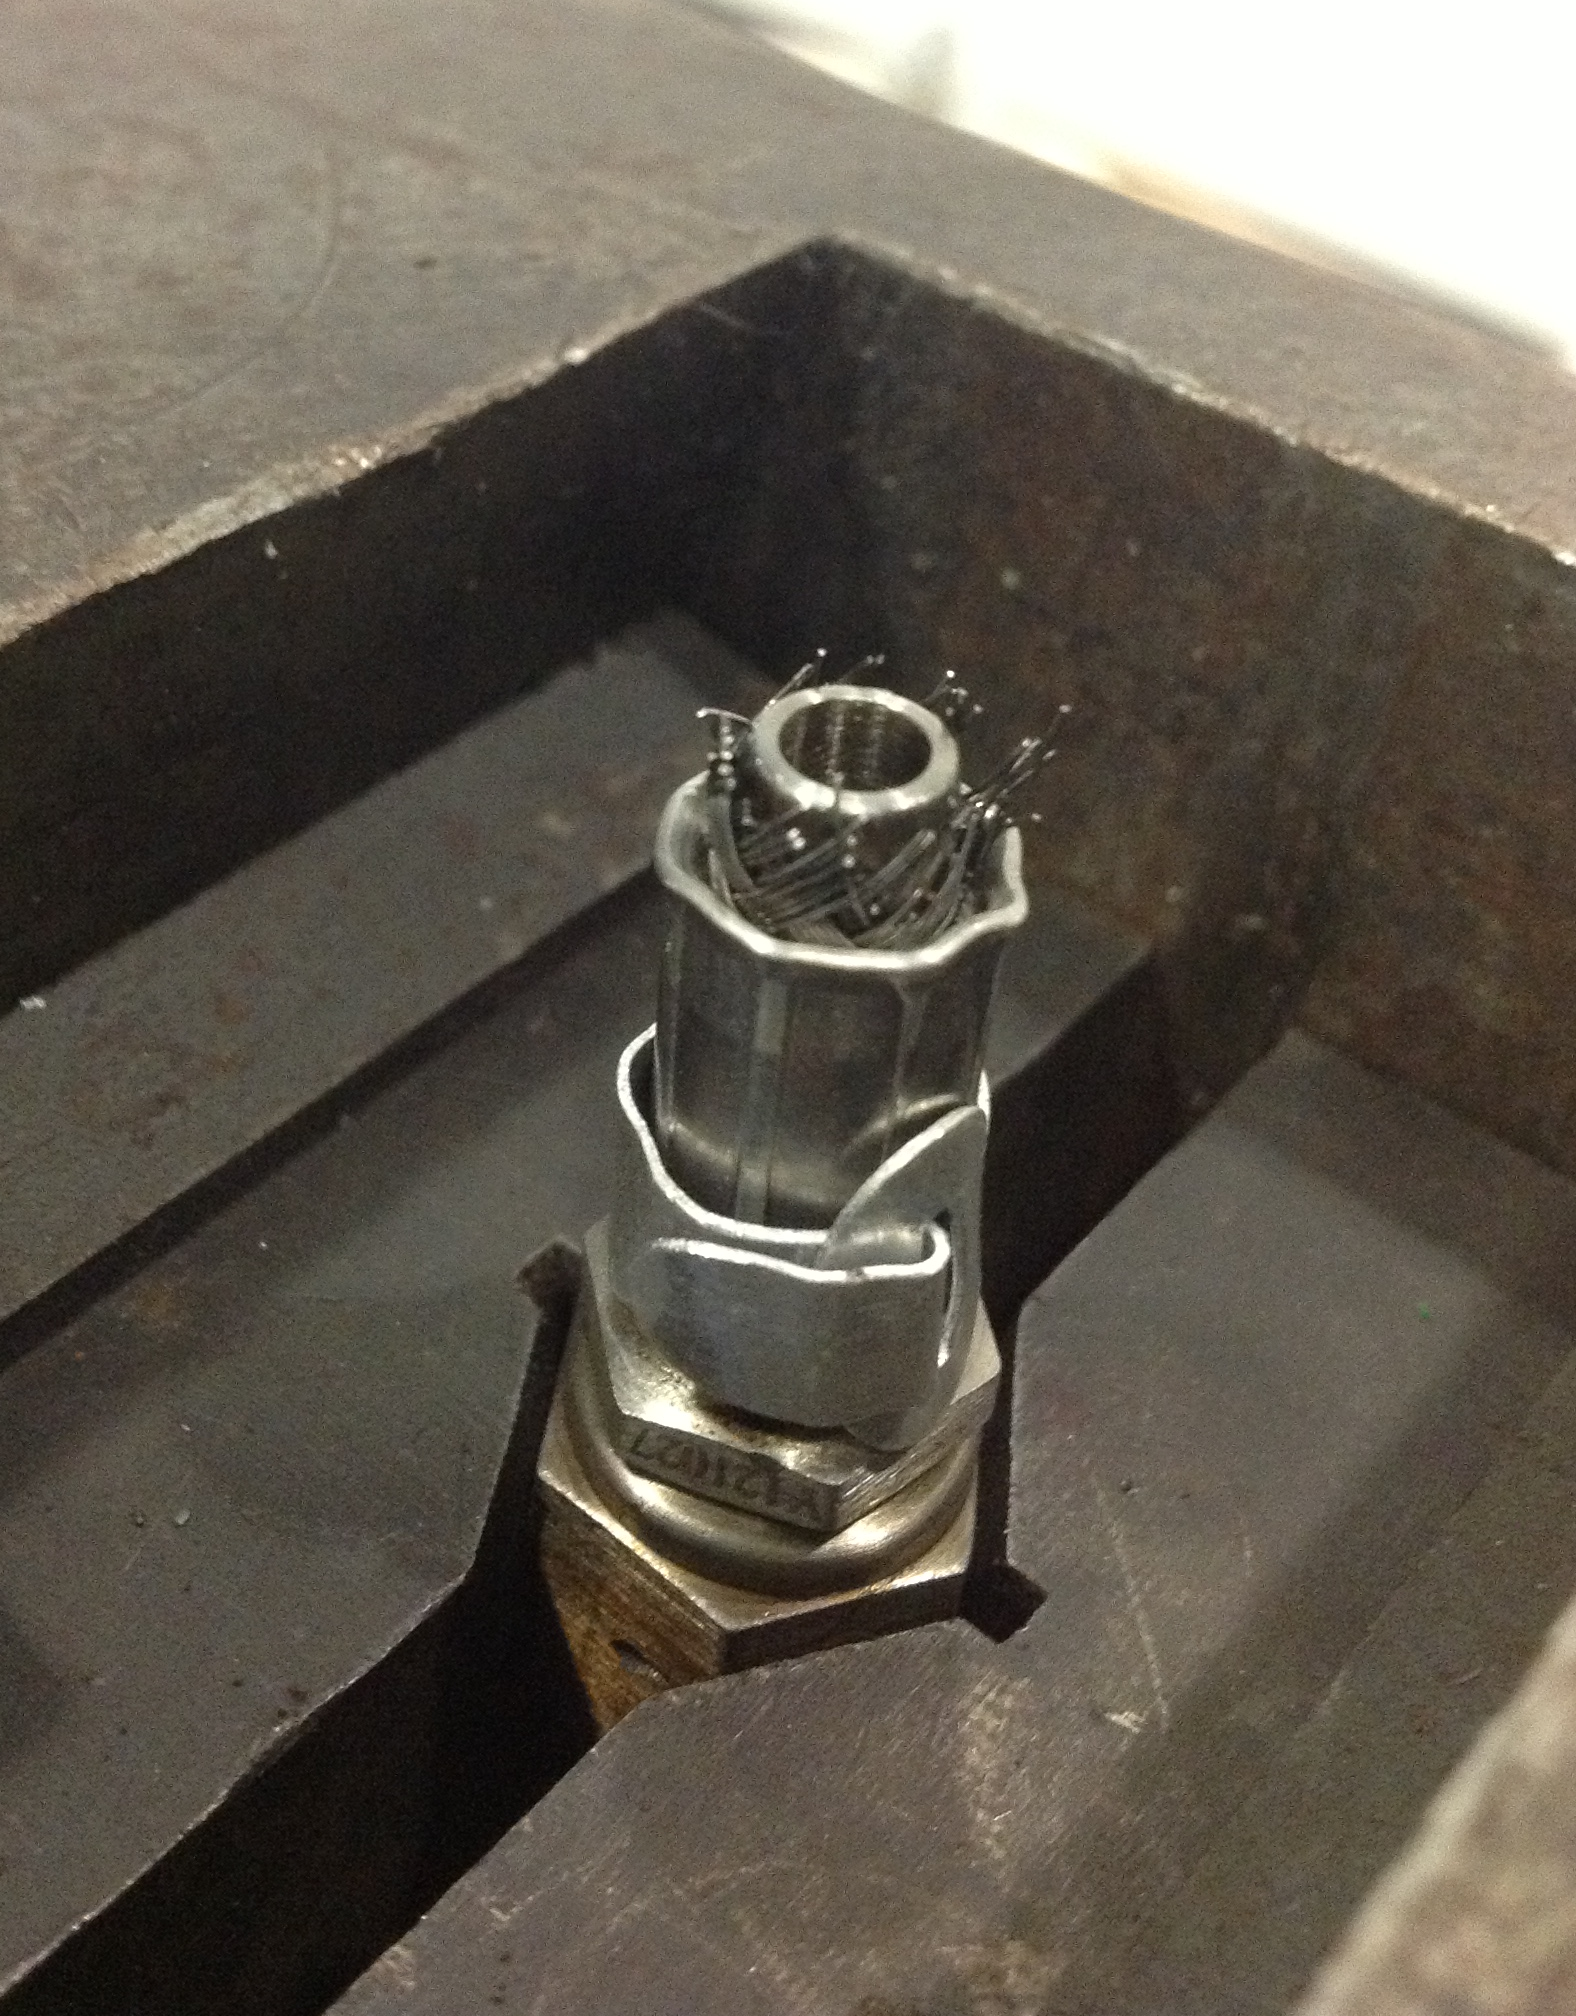
\includegraphics[height=0.2\textheight]{figure/experiment/E1/failure-1}}
	\hspace{0.5cm}
	\subfigure{
21		\includegraphics[height=0.2\textheight]{figure/experiment/E1/failure-2}}
	\hspace{0.5cm}
	\subfigure{
		\includegraphics[height=0.2\textheight]{figure/experiment/E1/necking}}
	\fcaption{破坏形式}{experiment-1:}
	\label{fig:experiment-1-fail}
\end{figure}









\section{第二次拉伸实验}
\subsection{试件参数}
第二次拉伸实验的软管试件包含了PTFE材质的内管,各项参数与普通使用的软管基本一致。同时实验进行了PTFE内管的拉伸实验,因为不同配方,不同烧制工艺会影响到PTFE材料的力学性能。
如图\ref{fig:tesile-experiment-II}所示 ,实验试件共4组,其中两组PTFE内管,两组为软管组件。

拉伸实验

\begin{table}[!htb]
	\centering
	\tcaption{实验试件}{Hose Specimen of the traction experiment}
	\label{tab:hose-specimen-II}
	\begin{tabular*}{0.8\textwidth}{@{\extracolsep{\fill}}>{\hspace{0.5cm}}ccc}
		\toprule
		&     软管组件-1     &     软管组件-2     \\ \midrule
		软管形式& 编织层+PTFE内管&编织层+PTFE内管\\
		编织层外径(mm)            &     7.60      &     7.59      \\
		内管内径 (mm)           &     4.99      &     5.01      \\
		软管长度 (mm)           &     420.0     &     421.5     \\
		编织角 (\textdegree) &     52.1      &     53      \\
		股数$ \times $根数    & 24$ \times $6 & 24$ \times $6 \\
		钢丝直径(mm)          &      0.2      &      0.2      \\ \bottomrule
	\end{tabular*} 
\end{table}

\begin{table}[!htb]
	\centering
	\tcaption{实验试件-2}{Hose Specimen of the traction experiment}
	\label{tab:hose-specimen-II-2}
	\begin{tabular*}{0.8\textwidth}{@{\extracolsep{\fill}}>{\hspace{0.5cm}}ccc}
		\toprule
		&     软管组件-1     &     软管组件-2     \\ \midrule
		软管形式& PTFE内管&PTFE内管\\
		外径(mm)            &     7.01      &     6.99      \\
		内径 (mm)           &     5.00      &     5.01      \\
		长度 (mm)           &     420.0     &     423     \\ \bottomrule
	\end{tabular*} 
\end{table}


\begin{figure}
\centering
\subfigure[]{
\includegraphics[height=0.18\textheight]{figure/experiment/E2/PTFE-inner-tube-1}
\label{fig:PTFE-inner-tube-1}
}
\hspace{0.5cm}
\subfigure[]{
\includegraphics[height=0.18\textheight]{figure/experiment/E2/PTFE-inner-tube-2}
\label{fig:PTFE-inner-tube-2}
}
\subfigure[]{
	\includegraphics[height=0.18\textheight]{figure/experiment/E2/PTFE-braid-tube-1}
	\label{fig:PTFE-braid-tube-1}
}
\hspace{0.5cm}
\subfigure[]{
	\includegraphics[height=0.18\textheight]{figure/experiment/E2/PTFE-braid-tube-2}
	\label{fig:PTFE-braid-tube-2}
}
\fcaption{第二次拉伸实验试件}{Hose Specimen}
\label{fig:tesile-experiment-II}
\end{figure}


\subsection{力位移曲线}
实验结果力位移曲线如图\ref{fig:tesile-experiment-II}所示,

\begin{figure}[!htb]
	\centering
	\includegraphics[width=0.6\textwidth]{figure/experiment/E2/Graph01}
	\subfigure[]{
			\includegraphics[width=0.4\textwidth]{figure/experiment/E2/Graph02}
			}
	\subfigure[]{
			\includegraphics[width=0.4\textwidth]{figure/experiment/E2/Graph03}
		}
	\fcaption{第二次拉伸实验}{experiment-2}  
	\label{fig:experiment-2}
\end{figure}


\subsection{破坏形式}



第二组带内管的试件的破坏形式如图\ref{fig:failure-experiment-ii}所示,编织层仍然在接头处钢丝断裂破坏。

\begin{figure}
\centering
\subfigure{
\includegraphics[height=0.3\textheight]{figure/experiment/E2/fail-1}
\label{fig:fail-1}
}
\hspace{1cm}
\subfigure{
\includegraphics[height=0.3\textheight]{figure/experiment/E2/fail-2}
\label{fig:fail-2}
}
\fcaption{破坏形式}{Failure}
\label{fig:failure-experiment-ii}
\end{figure}


\subsection{PTFE内管拉伸结果}

实验同时也确定了PTFE内管的力学性能,拉伸的力位移曲线如图\ref{fig:PTFE-traction},对比同口径带编织层的软管(图\ref{fig:PTFE}),可以观察到软管拉伸量较小,总体应变量小于0.06时,拉力主要由软管组件的内管承担。
\begin{figure}[!htb]
\centering
\subfigure[]{
\includegraphics[height=0.25\textheight]{figure/experiment/E2/PTFE}
\label{fig:PTFE-2}
}
\hspace{0.5cm}
\subfigure[]{
\includegraphics[height=0.25\textheight]{figure/experiment/E2/PTFE-2}
\label{fig:PTFE}
}
\fcaption{PTFE内管拉伸实验结果}{PTFE inner tube traction results}
\label{fig:PTFE-traction}
\end{figure}





\newpage
\section{第三次拉伸实验}
\subsection{试件参数}
  第三次拉伸实验对两个规格的PTFE软管组件进行了拉伸,分别类8mm口径和18mm口径。
  
  实验试件共分分为四组,8mm口径、18mm口径各两组,每组按不同编织密度制作试件分别为65\%、70\%、80\%、90\%,分别标记为BD-65、BD-70、BD-80、BD-90,BD代表编织密度(Braid Density)。各试件具体几何参数如表示\ref{tab:hose-specimen-III}所示。其中编织密度较低的试件,如BD-65、BD-70,按照正常流程还需要增加外套层保证结构稳定;本实验为了保证可以测量编织层编织角的变化,没有增加外套层。
  
  
%  试件参数
  
  \begin{table}[!htb]
  	\centering
  	\tcaption{实验试件}{Hose Specimen of the traction experiment}
  	\label{tab:hose-specimen-III}
  	\begin{tabular*}{0.8\textwidth}{@{\extracolsep{\fill}}>{\hspace{0.5cm}}ccccc}
  		\toprule
  		\textbf{第一组}&     BD-65     &     BD-70     &     BD-80     &     BD-90     \\ \midrule
  		编织层外径(mm)  & 26.8         &     24.63     &     22.06     &     19.22       \\
  		软管长度 (mm)    & 320          &      323      &      322      &      325       \\
  		编织角 (\textdegree)   & 46.76 &     48.22     &     47.41     &     53.56     \\
  		股数$ \times $根数          & 24$ \times $6 & 24$ \times $6 & 24$ \times $6 & 24$ \times $6 \\
  		钢丝直径(mm)                &      0.2      &      0.2      &      0.2      &      0.2      \\ \bottomrule
  	\end{tabular*} 
  \end{table}
  
  \begin{table}[!htb]
  	\centering

  	\begin{tabular*}{0.8\textwidth}{@{\extracolsep{\fill}}>{\hspace{0.5cm}}ccccc}
  		\toprule
  		\textbf{第二组}          &     BD-65     &     BD-70     &     BD-80     &     BD-90     \\ \midrule
  		编织层外径(mm)  & 27.23      &     26.23     &     20.48     &     22.8        \\
  		软管长度(mm)    & 319       &      322      &      322      &      321        \\
  		编织角(\textdegree)& 45.75 &     50.00     &     48.42     &     51.08      \\
  		股数$ \times $根数        & 24$ \times $6 & 24$ \times $6 & 24$ \times $6 & 24$ \times $6 \\
  		钢丝直径(mm)              &      0.2      &      0.2      &      0.2      &      0.2      \\ \bottomrule
  	\end{tabular*} 
  \end{table}
  
  \begin{table}[!htb]
  	\centering
  	\begin{tabular*}{0.8\textwidth}{@{\extracolsep{\fill}}>{\hspace{0.5cm}}ccccc}
  		\toprule
  		\textbf{第三组}       &     BD-65     &     BD-70     &     BD-80     &     BD-90     \\ \midrule
  		编织层外径(mm)  10.16   &     10.28     &     9.75      &     9.91      &     9.66      \\
  		软管长度(mm)    318    &      319      &      319      &      318      &      323      \\
  		编织角(\textdegree)32 &     43.66     &     46.62     &     47.82     &     51.03     \\
  		股数$ \times $根数     & 24$ \times $6 & 24$ \times $6 & 24$ \times $6 & 24$ \times $6 \\
  		钢丝直径(mm)           &      0.2      &      0.2      &      0.2      &      0.2      \\ \bottomrule
  	\end{tabular*} 
  \end{table}  

  \begin{table}[!htb]
  	\centering
  	\begin{tabular*}{0.8\textwidth}{@{\extracolsep{\fill}}>{\hspace{0.5cm}}ccccc}
  		\toprule
  		\textbf{第四组}          &     BD-65     &     BD-70     &     BD-80     &     BD-90     \\ \midrule
  		编织层外径(mm)  & 10.23      &     10.06     &      9.6      &      8.5        \\
  		软管长度(mm)    & 322       &      325      &      327      &      326        \\
  		编织角(\textdegree)& 42.58 &     44.96     &     49.90     &     50.24       \\
  		股数$ \times $根数        & 24$ \times $6 & 24$ \times $6 & 24$ \times $6 & 24$ \times $6 \\
  		钢丝直径(mm)              &      0.2      &      0.2      &      0.2      &      0.2      \\ \bottomrule
  	\end{tabular*} 
  \end{table}


\begin{figure*}
\centering
\includegraphics[height=0.25\textheight]{figure/experiment/18mm-hose-specimen}
\fcaption{实验试件}{hose specimen}
\label{fig:Slice1}
\end{figure*}


\subsection{实验结果}
本研究拉伸实验共进行三次,前两次采用的是摄影法,实验效果并不令人满意。只采用了相对较为准确的初始测量角,因其拍摄条件可控;第三次采用拓印法,记录的数据可靠可信,实验中不仅记录了初始编织角,还记录了过程中的编织角变化。

\begin{table}[!htb]
	\centering
	\tcaption{实验试件-2}{Hose Specimen of the traction experiment}
	\label{tab:hose-specimen-II-2}
	\begin{tabular}{@{\extracolsep{\fill}}>{\hspace{0.5cm}}ccccc}
		\toprule
		& 编织角测量方法 &   起始编织角    &  过程编织角变化   &   测量准确性    \\ \midrule
		拉伸实验 &   摄影法   & \checkmark &            &  \\
		拉伸实验 &   摄影法   & \checkmark &            &  \\
		拉伸实验 &   拓印法   & \checkmark & \checkmark & \checkmark \\ \bottomrule
	\end{tabular} 
\end{table}


\subsubsection{第一组试件}

第一组试件的位移曲线如图\ref{fig:E3-g1}所示,

\begin{figure}[!htb]
	\centering
	
	\subfigure{
		\includegraphics[height=0.35\textheight]{figure/experiment/E3-G1/Graph01}}
	\subfigure{
		\includegraphics[height=0.4\textheight]{figure/experiment/E3-G1/Graph02}}
	
	\fcaption{软管组件}{Hose Assembly}  
	\label{fig:E3-g1}
\end{figure}

\subsubsection{第二组试件}

第二组试件
\begin{figure}[!htb]
	\centering
	
	\subfigure{
		\includegraphics[height=0.35\textheight]{figure/experiment/E3-G2/Graph01}}
	\subfigure{
		\includegraphics[height=0.4\textheight]{figure/experiment/E3-G2/Graph02}}
	
	\fcaption{软管组件}{Hose Assembly}  
%	\label{fig:hose}
\end{figure}




\subsubsection{第三组试件}

第三组试件
\begin{figure}[!htb]
	\centering
	
	\subfigure{
		\includegraphics[height=0.35\textheight]{figure/experiment/E3-G3/Graph01}}
	\subfigure{
		\includegraphics[height=0.4\textheight]{figure/experiment/E3-G3/Graph02}}
	
	\fcaption{软管组件}{Hose Assembly}  
%	\label{fig:hose}
\end{figure}

\subsubsection{第四组试件}

第四组试件
\begin{figure}[!htb]
	\centering
	
	\subfigure{
		\includegraphics[height=0.35\textheight]{figure/experiment/E3-G4/Graph01}}
	\subfigure{
		\includegraphics[height=0.4\textheight]{figure/experiment/E3-G4/Graph02}}
	
	\fcaption{软管组件}{Hose Assembly}  
%	\label{fig:hose}
\end{figure}

\subsection{破坏形式}

各组试件接头处君发生接头脱头的现象,如图\ref{fig:fail-experiment-III},因此软管拉伸失效时,编织层钢丝有别与之前的两次实验,均为发生断裂如图\ref{fig:E3-hose-fail}所示。

\begin{figure}[!htb]
	\centering
	\subfigure{
		\includegraphics[height=0.25\textheight]{figure/experiment/E3-G3/Specimen/fail-2}
		\label{fig:fail-2}
	}
	\hspace{1cm}
	\subfigure{
		\includegraphics[height=0.25\textheight]{figure/experiment/E3-G3/Specimen/fail}
		\label{fig:fail}
	}
	\fcaption{破坏形式}{fail}
	\label{fig:fail-experiment-III}
\end{figure}


\begin{figure}[!htb]
	\centering
	\subfigure{
		\includegraphics[height=0.18\textheight]{figure/experiment/E3-G3/Specimen/fail-g1}
		\label{fig:fail-g1}
	}
	\hspace{0.5cm}
	\subfigure{
		\includegraphics[height=0.18\textheight]{figure/experiment/E3-G3/Specimen/fail-g2}
		\label{fig:fail-g2}
	}
	\hspace{0.5cm}
	\subfigure{
		\includegraphics[height=0.18\textheight]{figure/experiment/E3-G3/Specimen/fail-g3}
		\label{fig:fail}
	}
	\hspace{0.5cm}
	\subfigure{
		\includegraphics[height=0.18\textheight]{figure/experiment/E3-G3/Specimen/fail-g4}
		\label{fig:fail-g4}
	}
	\fcaption{第三组试件破坏形式}{hose fail}
	\label{fig:E3-hose-fail}
\end{figure}





\subsection{编织角变化}
如图\ref{fig:braid-angle-variation}所示,为各组试件中BD-90软管的编织角在拉伸中的变化。

\begin{figure}[!htb]
\centering
\subfigure[]{
\includegraphics[height=0.22\textheight]{figure/experiment/g1-90}
\label{fig:g1-90}
}
\subfigure[]{
\includegraphics[height=0.22\textheight]{figure/experiment/g2-90}
\label{fig:g2-90}
}
\subfigure[]{
\includegraphics[height=0.22\textheight]{figure/experiment/g3-90}
\label{fig:g3-90}
}
\subfigure[]{
\includegraphics[height=0.22\textheight]{figure/experiment/g4-90}
\label{fig:g4-90}
}
\fcaption{编织角变化}{Braid Angle Variation}
\label{fig:braid-angle-variation}
\end{figure}



\begin{figure*}[!htb]
\centering
%\subfigure{
%\includegraphics[width=0.3\textwidth]{figure/experiment/braid-angle/g1-65}
%\label{fig:g1-65}
%}
\subfigure{
\includegraphics[width=0.3\textwidth]{figure/experiment/braid-angle/g1-70}
\label{fig:g1-70}
}
\subfigure{
\includegraphics[width=0.3\textwidth]{figure/experiment/braid-angle/g1-80}
\label{fig:g1-80}
}
\subfigure{
\includegraphics[width=0.3\textwidth]{figure/experiment/braid-angle/g1-90}
\label{fig:g1-90-2}
}
\fcaption{}{}
\label{fig:g1-braid-angle}
\end{figure*}















\section{实验结果分析}

本研究拉伸实验得到了几组试件拉伸的力位移曲线,结果与
\citeauthor{Hachemi2011}试件的拉伸结果一致,都体现出了软管组件编织层受拉时的非线性力学行为。


\begin{figure}[!htb]
	\centering
	\includegraphics[height=0.25\textheight]{figure/experiment/Hachemi-Result-ex}
	\fcaption{Hachemi实验试件}{Hachemi Hose Specimen}
	\label{fig:Hachemi-Result-ex}
\end{figure}

图\ref{fig:Hachemi-Result-ex}为其实验拉伸的力位移曲线,图中有两个明显的拐点。a处拐点理论认为是由编织角的变化引起的的;b处拐点\cite{Hachemi2011}给出了假设:
\begin{compactenum}
\item 编织层的空隙在拉伸中被填满,编织角不能继续变化导致了力位移曲线出现了拐点,称之为锁定角;
\item 进一步拉伸时,编织层中的钢丝发生了塑性变形。
\end{compactenum}




\begin{figure*}[!htb]
\centering
\subfigure[]{
	\includegraphics[height=0.17\textheight]{figure/experiment/hachemi-hyper-3}
	\label{fig:hachemi-hyper-3}
}
\subfigure[]{
	\includegraphics[height=0.15\textheight]{figure/experiment/braid-gap}
}
\subfigure[]{
\includegraphics[height=0.22\textheight]{figure/experiment/hachemi-hyper-1}
\label{fig:hachemi-hyper-1}
}
\subfigure[]{
	\includegraphics[height=0.22\textheight]{figure/experiment/hachemi-hyper-2}
	\label{fig:hachemi-hyper-2}
}
\fcaption{Hachemi锁定编织角假设}{Hachemi's hypothesis of braid angle lock}
\label{fig:hachemi-hyper}
\end{figure*}


\citeauthor{Hachemi2011}还给出了锁定角的计算方法:图\ref{fig:hachemi-hyper-1}中的特征单元中,
$ AC = 4\pi D/{N_S} $,$ AD =  $
当空隙面积$ S=0 $时,$ AC = AD/2 $,即








\begin{equation}
\frac{{2\pi D}}{{{N_S}}} = \frac{{{N_W}\phi }}{{\cos \alpha }}
\end{equation}

\begin{equation}
\label{eq:lockalpha}
{\alpha _{lock}} = \arccos \frac{{{N_S}{N_W}\phi }}{{2\pi D}}
\end{equation}

根据该假设,软管组件在拉伸实验过程中,当编织角小于$ \alpha_lock $时,就会锁定不变。

本实验根据拉伸实验的测试结果,针对了以上假设,深入分析了一下两个命题:
\begin{compactitem}
	\item \textbf{编织角是否会锁定?}
	\item \textbf{金属纤维是否发生塑性应变?}
\end{compactitem}





\subsubsection{编织角不锁定}

第三次拉伸实验所记录的拉伸过程中编织角变化,可以比较明显的观察到,力位移曲线在发生非线性的变化是,编织角是保持变化的。如图\ref{fig:angle-conclusion}所示,该组实验中对编织角的采样较为密集,可以清楚的看到编织角保持着减小的趋势;可见编织角不会发生锁定。根据\ref{eq:lockalpha}计算该试件的$ \alpha_{lock} $为$ 38.43\textdegree $,而实验中试件的编织角持续较小,达到$ 32.16\textdegree $。

\begin{figure}[!htb]
	\centering
	\subfigure[]{
		\includegraphics[height=0.22\textheight]{figure/experiment/g1-90}
		\label{fig:g1-90}
	}
	\fcaption{编织角变化}{Braid Angle Variation}
	\label{fig:angle-conclusion}
\end{figure}

观察实验采集的各组试件编织角的数据,发现编织角基本上呈线性变化, 对其进行线性拟合,各组编织角拟合的趋势线均能较好的吻合实验数据结果。




\subsubsection{金属纤维不发生塑性应变}



在3次试验中挑选典型试验结果进行比对,如表\ref{tab:hose-comparation}所示,拉伸的力位移曲线如图\ref{fig:hose-comparation}所示。

\begin{table}[!htb]
	\centering
	\tcaption{实验试件-2}{Hose Specimen of the traction experiment}
	\label{tab:hose-comparation}
	\begin{tabular}{@{\extracolsep{\fill}}>{\hspace{0.5cm}}cccc}
		\toprule
		实验组别 & 试件编号& 软管组件形式& 破坏形式\\\midrule
		实验I& 芯棒1& 编织层& 接头钢丝断裂\\
		实验II& 软管组件2& 编织层+内管& 接头钢丝断裂\\
		实验III& 第一组-BD-80& 编织层+内管& 接头脱头\\\bottomrule
	\end{tabular} 
\end{table}  


\begin{figure}[!htb]
	\centering
	\subfigure[]{
		\includegraphics[height=0.22\textheight]{figure/chap2/plasiticity-3}
		\label{fig:hose-comparation-1}}
	\subfigure[]{
		\includegraphics[height=0.22\textheight]{figure/chap2/plasiticity-2}
		\label{fig:hose-comparation-2}}
	\subfigure[]{
		\includegraphics[height=0.22\textheight]{figure/chap2/plasiticity-1}
		\label{fig:hose-comparation-3}}
	\fcaption{试件对比}{}
	\label{fig:hose-comparation}
\end{figure}





图\ref{fig:hose-comparation-1}中,试件的力位移曲线没有出现类似Hachemi试件的拐点,实验中观察不到钢丝发生塑性应变;断裂时现象类似脆断。由于编织层采用的钢丝断裂伸长率仅为约$ 2\% $,可以解释以上现象。
图\ref{fig:hose-comparation-2}中,力位移曲线轻微偏离非线性增长的趋势,直到最后组件发生脆断。
图\ref{fig:hose-comparation-3}中,试件的力位移曲线较大偏离了非线性增长的趋势。而偏离段的实验过程中,可以发现软管组件接头扣压逐渐松脱;虽然没有出现类似Hachemi试件的拐点,但是曲线的趋势有明显的变化。

综合分析这些实验现象和实验数据,本研究认为:编织层采用断裂伸长率较小的钢丝时,钢丝轻微的塑性变形不会导致编织层结构在拉伸时,出现刚度降低的拐点。拐点的出现更有可能的原因是:接头扣压随着软管内管管壁在拉伸过程中逐渐变薄而逐渐失效,接头中的钢丝逐渐从扣押的约束中释放导致刚度降低;钢丝完全释放则软管发生脱头现象,不完全释放则在钢丝到达极限伸长量时断裂。



\section{小~结}
